\subsection{Architecture Overview}

The MicroNet framework is a collection of components. Each component is confined
in itself which allows simple replacement of components. The components are
organized in three component groups referred to as features: the framework
feature, the service catalogue feature, and the tools feature.
\autoref{fig:architecture_layers} shows the relation of the features and all the
components they contain.

The features and the components they contain are explained below using Component
Responsibility Cards (CRC).

\begin{figure}
  \centering
  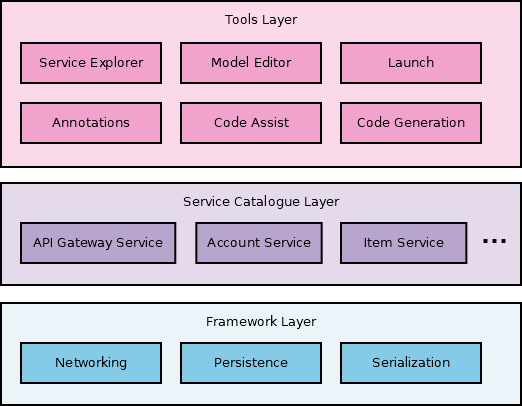
\includegraphics[width=0.8\textwidth]{images/architecture/ArchitectureLayers}
  \caption{The features of MicroNet with the associated components.}
  \label{fig:architecture_layers}
\end{figure}

\subsubsection{Framework Feature}

The framework feature provides a uniform interface to the core functionality of
MicroNet.\\

\noindent
\begin{tabular}{|l|l|}
    \cline{1-2}
    \multicolumn{2}{|c|}{} \\[-0.3cm]
    \multicolumn{2}{|c|}{Networking Component} \\ 
    \multicolumn{2}{|c|}{} \\[-0.3cm]
    \cline{1-2}
    Responsibility & Collaboration \\
    \cline{1-2}
    & \\[-0.2cm]
    \begin{minipage}{0.47\textwidth}
        \begin{itemize}
          \item Provide an interface to the reliable messaging system
          \item Correlate users and connection
          \item Expose the Java \textit{Messaging API}
        \end{itemize} 
    \end{minipage}
	&
    \begin{minipage}{0.47\textwidth}
        \begin{itemize}
          \item Message Broker (ActiveMQ)
          \item Serialization Component
        \end{itemize} 
    \end{minipage}
	\\ & \\
    \hline
\end{tabular}

\vspace{0.5cm} \noindent 
\begin{tabular}{|l|l|}
    \cline{1-2}
    \multicolumn{2}{|c|}{} \\[-0.3cm]
    \multicolumn{2}{|c|}{Persistence Component} \\ 
    \multicolumn{2}{|c|}{} \\[-0.3cm]
    \cline{1-2}
    Responsibility & Collaboration \\
    \cline{1-2}
    & \\[-0.2cm]
    \begin{minipage}{0.47\textwidth}
        \begin{itemize}
          \item Provide uniform database access
          \item Offer relational database
          \item Offer NoSQL database
          \item Expose the Java database \gls{api}
        \end{itemize} 
    \end{minipage}
	&
    \begin{minipage}{0.47\textwidth}
        \begin{itemize}
          \item Relational DBMS (PostgreSQL)
          \item JDBC
          \item NoSQL Database (Couchbase)
        \end{itemize} 
    \end{minipage}
	\\ & \\
    \hline
\end{tabular}

\vspace{0.5cm} \noindent 
\begin{tabular}{|l|l|}
    \cline{1-2}
    \multicolumn{2}{|c|}{} \\[-0.3cm]
    \multicolumn{2}{|c|}{Serialization Component} \\ 
    \multicolumn{2}{|c|}{} \\[-0.3cm]
    \cline{1-2}
    Responsibility & Collaboration \\
    \cline{1-2}
    & \\[-0.2cm]
    \begin{minipage}{0.47\textwidth}
        \begin{itemize}
          \item Expose the uniform serialization \gls{api}
          \item Make the serialization technology interchangeable
          \item Provide \gls{json} serialization
          \item Provide binary serialization
        \end{itemize} 
    \end{minipage}
	&
    \begin{minipage}{0.47\textwidth}
        \begin{itemize}
          \item Serialization Library (Gson)
        \end{itemize} 
    \end{minipage}
	\\ & \\
    \hline
\end{tabular}

\subsubsection{Service Catalogue Feature}

The service catalogue was mainly developed in the second semester thesis
\cite{biedermann2016project2} in Chapter 5 Prototype Implementation.
This section will give three representative examples of catalogue services.\\

\noindent
\begin{tabular}{|l|l|}
    \cline{1-2}
    \multicolumn{2}{|c|}{} \\[-0.3cm]
    \multicolumn{2}{|c|}{API Gateway Service} \\ 
    \multicolumn{2}{|c|}{} \\[-0.3cm]
    \cline{1-2}
    Responsibility & Collaboration \\
    \cline{1-2}
    & \\[-0.2cm]
    \begin{minipage}{0.47\textwidth}
        \begin{itemize}
          \item Receive and filter requests from clients
          \item Forward requests to \mss{}
          \item Forward events to clients
          \item Broadcast events to groups of clients
        \end{itemize} 
    \end{minipage}
	&
    \begin{minipage}{0.47\textwidth}
        \begin{itemize}
          \item Account Service (connection authentication)
        \end{itemize} 
    \end{minipage}
	\\ & \\
    \hline
\end{tabular}

\vspace{0.5cm} \noindent 
\begin{tabular}{|l|l|}
    \cline{1-2}
    \multicolumn{2}{|c|}{} \\[-0.3cm]
    \multicolumn{2}{|c|}{Account Service} \\ 
    \multicolumn{2}{|c|}{} \\[-0.3cm]
    \cline{1-2}
    Responsibility & Collaboration \\
    \cline{1-2}
    & \\[-0.2cm]
    \begin{minipage}{0.47\textwidth}
        \begin{itemize}
          \item Process user registrations
          \item Process user authentications
        \end{itemize} 
    \end{minipage}
	&
    \begin{minipage}{0.47\textwidth}
        \begin{itemize}
          \item Account Database (PostgreSQL)
        \end{itemize} 
    \end{minipage}
	\\ & \\
    \hline
\end{tabular}

\vspace{0.5cm} \noindent 
\begin{tabular}{|l|l|}
    \cline{1-2}
    \multicolumn{2}{|c|}{} \\[-0.3cm]
    \multicolumn{2}{|c|}{Item Service} \\ 
    \multicolumn{2}{|c|}{} \\[-0.3cm]
    \cline{1-2}
    Responsibility & Collaboration \\
    \cline{1-2}
    & \\[-0.2cm]
    \begin{minipage}{0.47\textwidth}
        \begin{itemize}
          \item Provide access to player inventories (carried items)
          \item Provide access to player banks (item storage)
        \end{itemize} 
    \end{minipage}
	&
    \begin{minipage}{0.47\textwidth}
        \begin{itemize}
          \item Item Database (PostgreSQL)
        \end{itemize} 
    \end{minipage}
	\\ & \\
    \hline
\end{tabular}

\subsubsection{Tools Feature}

The development of the tools feature was a major part of the \gls{dsm} lab
research. The tools feature's main purpose is to provide support for the tenet
decentralized continuous delivery. But the tools feature also has the
responsibility to adapt the \ms{} application development process to be suitable
for \og{} development.\\

\noindent
\begin{tabular}{|l|l|}
    \cline{1-2}
    \multicolumn{2}{|c|}{} \\[-0.3cm]
    \multicolumn{2}{|c|}{Annotation Processing} \\ 
    \multicolumn{2}{|c|}{} \\[-0.3cm]
    \cline{1-2}
    Responsibility & Collaboration \\
    \cline{1-2}
    & \\[-0.2cm]
    \begin{minipage}{0.47\textwidth}
        \begin{itemize}
          \item Provide an entrypoint for the framework
          functionality\footnotemark
          \item Help to reduce boilerplate code 
          \item Define the \textit{Service API}
        \end{itemize} 
    \end{minipage}
	&
    \begin{minipage}{0.47\textwidth}
        \begin{itemize}
          \item Shared Model (to export the \gls{api})
        \end{itemize} 
    \end{minipage}
	\\ & \\
    \hline
\end{tabular}

\footnotetext{The user code is
          called by the framework (application skeleton) as opposed to the user
          code calling a library (well-defined operations).}
          
\vspace{0.5cm} \noindent      
\begin{tabular}{|l|l|}
    \cline{1-2}
    \multicolumn{2}{|c|}{} \\[-0.3cm]
    \multicolumn{2}{|c|}{Code Assist} \\ 
    \multicolumn{2}{|c|}{} \\[-0.3cm]
    \cline{1-2}
    Responsibility & Collaboration \\
    \cline{1-2}
    & \\[-0.2cm]
    \begin{minipage}{0.47\textwidth}
        \begin{itemize}
          \item Present the \textit{Service API} to the developer
          \item Show auto-completion of URIs
          \item Recognize \gls{api} usage errors at compile-time
        \end{itemize} 
    \end{minipage}
	&
    \begin{minipage}{0.47\textwidth}
        \begin{itemize}
          \item Shared Model (to import the \gls{api})
        \end{itemize} 
    \end{minipage}
	\\ & \\
    \hline
\end{tabular}

\vspace{0.5cm} \noindent         
\begin{tabular}{|l|l|}
    \cline{1-2}
    \multicolumn{2}{|c|}{} \\[-0.3cm]
    \multicolumn{2}{|c|}{Code Generation} \\ 
    \multicolumn{2}{|c|}{} \\[-0.3cm]
    \cline{1-2}
    Responsibility & Collaboration \\
    \cline{1-2}
    & \\[-0.2cm]
    \begin{minipage}{0.47\textwidth}
        \begin{itemize}
          \item Generate the MicroNet framework integration classes
          \item Generate POJOs from the \textit{Shared Model}
        \end{itemize} 
    \end{minipage}
	&
    \begin{minipage}{0.47\textwidth}
        \begin{itemize}
          \item Shared Model (to import the \gls{api} and Template Types)
          \item Java compiler (annotation processing)
        \end{itemize} 
    \end{minipage}
	\\ & \\
    \hline
\end{tabular}

\vspace{0.5cm} \noindent         
\begin{tabular}{|l|l|}
    \cline{1-2}
    \multicolumn{2}{|c|}{} \\[-0.3cm]
    \multicolumn{2}{|c|}{Service Explorer} \\ 
    \multicolumn{2}{|c|}{} \\[-0.3cm]
    \cline{1-2}
    Responsibility & Collaboration \\
    \cline{1-2}
    & \\[-0.2cm]
    \begin{minipage}{0.47\textwidth}
        \begin{itemize}
          \item Provide a visual management interface for the application (UI)
          \item Compose the application out of catalogue and developed game
          services
        \end{itemize} 
    \end{minipage}
	&
    \begin{minipage}{0.47\textwidth}
        \begin{itemize}
          \item Service Catalogue
          \item Launch Utility (to provide the UI)
        \end{itemize} 
    \end{minipage}
	\\ & \\
    \hline
\end{tabular}

\vspace{0.5cm} \noindent      
\begin{tabular}{|l|l|}
    \cline{1-2}
    \multicolumn{2}{|c|}{} \\[-0.3cm]
    \multicolumn{2}{|c|}{Model Editor} \\ 
    \multicolumn{2}{|c|}{} \\[-0.3cm]
    \cline{1-2}
    Responsibility & Collaboration \\
    \cline{1-2}
    & \\[-0.2cm]
    \begin{minipage}{0.47\textwidth}
        \begin{itemize}
          \item Define and edit the \textit{Template
          Types} of the \textit{Shared Model} 
          \item Instantiate \textit{Template Types} as \textit{Prefabs}
          \item Synchronize the \textit{Shared Model} between developers
        \end{itemize} 
    \end{minipage}
	&
    \begin{minipage}{0.47\textwidth}
        \begin{itemize}
          \item Shared Model (CRUD)
          \item Database Component (for sharing)
        \end{itemize} 
    \end{minipage}
	\\ & \\
    \hline
\end{tabular}

\vspace{0.5cm} \noindent        
\begin{tabular}{|l|l|}
    \cline{1-2}
    \multicolumn{2}{|c|}{} \\[-0.3cm]
    \multicolumn{2}{|c|}{Launch Utility} \\ 
    \multicolumn{2}{|c|}{} \\[-0.3cm]
    \cline{1-2}
    Responsibility & Collaboration \\
    \cline{1-2}
    & \\[-0.2cm]
    \begin{minipage}{0.47\textwidth}
        \begin{itemize}
          	\item Build the composed application
			\item Simplify application deployment
          	\item Provide launch configurations for local deployments 
        \end{itemize} 
    \end{minipage}
	&
    \begin{minipage}{0.47\textwidth}
        \begin{itemize}
          \item Maven (build)
          \item Docker (build \& run)
          \item Docker-compose (compose the application)
          \item Optional use of CDT Launch Groups and Eclipse Docker Tools
        \end{itemize} 
    \end{minipage}
	\\ & \\
    \hline
\end{tabular}
